%!TEX root = ../report.tex

% 
% Related work
% 

\section{Related Work}

% Example citation:
In this section we will present a set of literature references on the subjects related to this thesis. We will present the most important frameworks on Information Systems Management and Governance. This process has the objective to come up with a choice of a frameworks or a set of them to implement our processes for project and maintenance management\par
In terms of logical application architectures, we will provide an analysis of the main features of a set of Project Management and Information Technologies Service Management solutions available in the market. Our objective is to conduct an comparative analysis relating all the solutions and choose the ones that best fit our purposes for use on an logical application architecture.  

\subsection{Frameworks for Information Technologies Governance and Management}

In this section we will present the three frameworks we consider the most relevant for this thesis: COBIT 5, ITIL V3 and PMBOK. This three frameworks provide, from different perspectives, guides and principles for IT Governance and Management, providing processes for achieving a successful implementation of this principles in an organization.\par


\subsubsection{IT Governance and IT Management}

One important concept to define is the difference between IT Governance and IT management. They are many times confused and some authors already tried to explain the difference between the two concepts.\par
Considering the definition given by Van Grembergen \textit{et al.}, ``''IT Management is focused on the internal effective supply of IT services and products and the management of present IT operations. IT Governance in turn is much broader, and concentrates on performing and transforming IT to meet present and future demands of the business (internal focus) and the business' customers (external focus).``''.\par
 Considering the COBIT 5 view for this question, it makes a clear distinction between governance and management, in the way these two disciplines encompass different types of activities, require different organizational structures and serve different purposes.\par
 Governance ensures that stakeholder needs, conditions and options are evaluated to determine balanced, agreed-on enterprise objectives to be achieved; setting direction through prioritisation and decision making; and monitoring performance and compliance against agreed-on direction and objectives.Management plans, builds, runs and monitors activities in alignment with the direction set by the governance body to achieve the enterprise objectives.\par

\begin{figure}
\centering
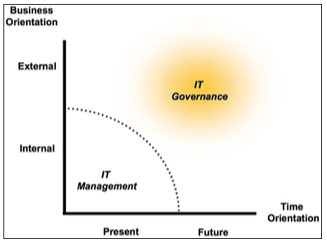
\includegraphics[width=0.6\textwidth]{img/ITGovernanceAndManagement.png}
\caption{IT Governance and IT Management}
\end{figure}


 Considering both definitions and the figure 1, we can conclude that IT Governance has a bigger dimension that IT Management, but are disciplines that need to be related and complementary to achieve success inside an organization.

\subsubsection{COBIT 5}

Control Objectives for Information and Related Technology (COBIT) is a framework created by the Information Systems Audit and Control Association (ISACA) for IT Management and IT Governance.\par
COBIT 5 provides a comprehensive framework that assists enterprises in achieving their objectives for the governance and management of enterprise IT. Simply stated, it helps enterprises create optimal value from IT by maintaining a balance between realizing benefits and optimizing risk levels and resource use \cite{2012cobit}. 
The framework is built on five basic principles:

\begin{itemize}
  \item Meeting the Stakeholders Needs 
  \item Covering the Enterprise End-to-end
  \item Applying a Single, Integrated Framework
  \item Enabling a Holistic Approach
  \item Separating Governance from Management
\end{itemize}


It also defines seven enablers, explained by COBIT as factors that, individually and collectively, influence whether governance and management over enterprise will work or not. This enablers can be categorized as:

\begin{itemize}
  \item Principles, Policies and frameworks 
  \item Processes 
  \item Organizational structures
  \item Culture, ethics and behavior 
  \item Information
  \item Services, infrastructure and applications
  \item People, skills and competencies
\end{itemize}

\begin{figure}
\centering
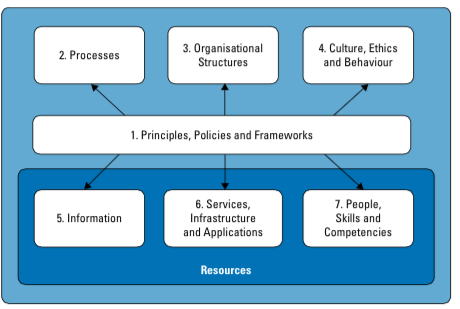
\includegraphics[width=0.7\textwidth]{img/Enablers.png}
\caption{COBIT 5 enablers}
\end{figure}

Image 2 presents the COBIT 5 enablers previous defined and how they relate among themselves int terms of its importance for organization. Each enabler has stakeholders, a set of goals, a life cycle and for each can be defined good practices.\par

\begin{figure}
\centering
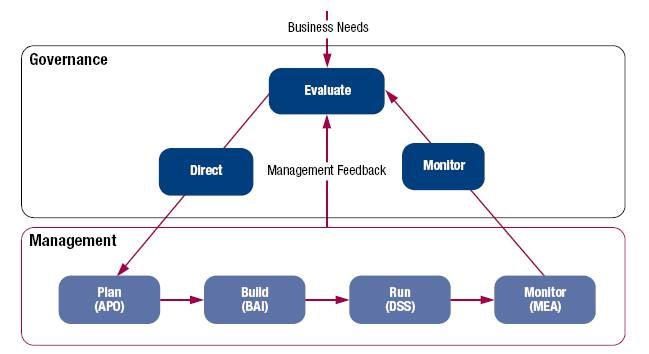
\includegraphics[width=0.9\textwidth]{img/COBITProcesses.jpg}
\caption{COBIT 5 domains}
\end{figure}

Considering figure 3, COBIT 5 process reference model considers two big domains of processes: Governance and Management. The governance domain contains five processes in the domain evaluate, direct and monitor(EDM). The management domain has four internal domains of processes:Align, Plan and Organise(APO), Build, Acquire and Implement(BAI), Deliver, Service and Support (DSS) and Monitor, Evaluate and Assess(MEA).\par
All processes for management and governance are presented in the appendix and all the implementation details explained in COBIT 5: Enabling Processes, A detailed reference guide to the processes defined in the COBIT 5 process reference model. This includes the COBIT 5 goals cascade, a process model explanation, governance and management practices, and the process reference model\cite{2012cobitEP}.\par
COBIT 5 includes a process capability model based on ISO/IEC 15504 Software Engineering - Process Assessment standard. [REFERENCE HERE] This models allow to measure the current level of maturity of enterprise processes, presenting the gap between the current level and the desired one the enterprise wants to achieve. This new capability model is an improvement of the previous on COBIT 4.1, being more simplified and compliant with a generally accepted process assessment standard.\par
Relating to other frameworks and standards, COBIT tries to establish a framework that is compliant with the most widely accepted standards in IT Governance and Management. In figure 4 we can see the standards COBIT 5 relates by processes domain, with special attention to ITIL V3, ISO/IEC 20000, PMBOK and CMMI, that are closely related to this thesis problem. This compliance with other standards is fundamental for a widely adoption of COBIT 5, in the way it tries to establish goals, metrics, practices, roles, inputs and outputs for each process, making it necessary being compliant with international standards. This is will improve COBIT application and acceptance.\par

\subsubsection{COBIT 5 critical analysis}

The COBIT 5 is one of the most interesting frameworks widely accepted by organizations in the IT management and Governance Area. It arises as the main framework for establishing processes to guide us on management and governance and establish ways to control them. However, its a complex framework that needs time and practice to be fully implemented.\par
For this thesis project, we will consider only the domains relevant for our objectives, making a selection of the processes we pretend to implement. This will allow us to get the bigger value COBIT has to offer, making it possible, in the time-frame available, achieve our implementation objectives.\par
One important aspect of the use of COBIT is that it provides a more business and strategic view of IT on organizations, presenting a lack of operational approach to some themes that are relevant for our project. To overcome this, we will analyze a more operational framework on IT service management, the ITIL V3 framework and a project management guide considered by the main specialists on the area as the reference for project management, the Project Management Book of Knowledge.\par

\begin{figure}
\centering
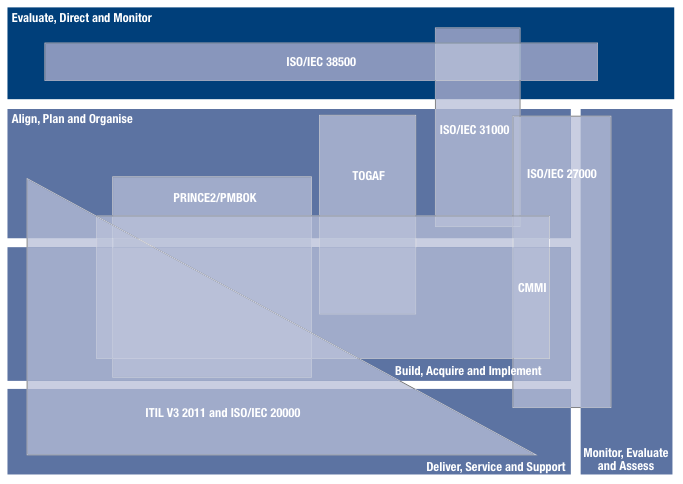
\includegraphics[width=0.9\textwidth]{img/COBITOtherFrameworks.png}
\caption{COBIT 5 coverage on other frameworks}
\end{figure}

\subsubsection{ITIL V3}

First developed in the 1980s by the Office of Government Commerce (OGC), a branch of the British Government, ITIL defines processes at a high level. It is left to the organizations to implement the processes in the manner most suitable to their particular situations and needs.\par
ITIL is becoming a de facto standard worldwide as organizations adopt it as their guideline for establishing IT service management (ITSM) processes. IT organizations can use the guidance provided by ITIL to transform their service management capabilities into strategic assets, those that provide the basis for core competence, distinctive performance, durable advantage, and qualifications to participate in business opportunities.\par
The ITIL service management practices are comprised of three main sets of products and services: ITIL service management practices (core guidance), ITIL service management practices (guidance specific to industry sectors, organization types, operating models and technology architectures) and ITIL web support services.\par

\begin{figure}
\centering
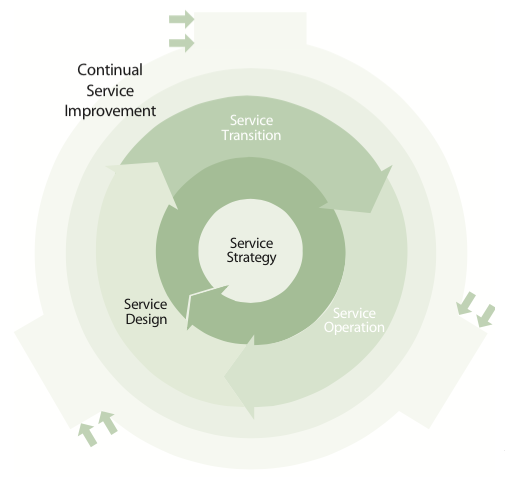
\includegraphics[width=0.7\textwidth]{img/ITILVolumes.png}
\caption{COBIT 5 coverage on other frameworks}
\end{figure}

The core set, presented in figure XXX and the one we will consider for this thesis, consists of six publications: Introduction to ITIL Service Management Practices, Service Strategy, Service Design, Service Transition, Service Operation and Continual Service Improvement. Each one of this volumes is composed by practice fundamentals and principles, Lifecycle processes and activities, Supporting organization structures and roles, Technology considerations, Practice implementation and Challenges, risks and critical success factors.

\paragraph{\textbf{Service Strategy}} provides guidance on how to view service management not only as an organizational capability but as a strategic asset. Guidance is provided on the principles underpinning the practice of service management which are useful for developing service management policies, guidelines and processes across the ITIL Service Lifecycle. The processes included in Service Strategy volume are:

\begin{itemize}
  \item Financial Management
  \item Service Portfolio Management 
  \item Demand Management
\end{itemize}

\paragraph{\textbf{Service Design}} provides guidance for the design and development of services and service management practices. It covers design principles and methods for converting strategic objectives into portfolios of services and service assets. The scope of Service Design is not limited to new services. It includes the changes and improvements necessary to increase or maintain value to customers over the lifecycle of services, the continuity of services, achievement of service levels, and conformance to standards and regulations. The processes included in Service Design volume are:

\begin{itemize}
  \item Service Catalogue Management
  \item Service Level Management 
  \item Capacity Management
  \item Availability Management
  \item IT service Continuity Management
  \item Information Security Management 
  \item Supplier Management
  \item Application Management
  \item Data and Information Management
  \item Business Service Management
\end{itemize} 

\paragraph{\textbf{Service Transition}} provides guidance for the development and improvement of capabilities for transitioning new and changed services into live service operation. This publication provides guidance on how the requirements of Service Strategy encoded in Service Design are effectively realized in Service Operation while controlling the risks of failure and disruption.The processes included in Service Transition volume are:

\begin{itemize}
  \item Change Management
  \item Service asset and Configuration Management
  \item Release and deployment Management
  \item Knowledge Management
  \item Stakeholder Management
  \item Transition Planning 
  \item Support and Service Evaluation 
\end{itemize} 

\paragraph{\textbf{Service Operation}} embodies practices in the management of the day-to-day operation of services. It includes guidance on achieving effectiveness and efficiency in the delivery and support of services to ensure value for the customer and the service provider. Strategic objectives are ultimately realized through Service Operation, therefore making it a critical capability. Guidance is provided on how to maintain stability in service operations, allowing for changes in design, scale, scope and service levels.The processes included in Service Operation volume are:

\begin{itemize}
  \item Event Management
  \item Incident Management
  \item Request Management
  \item Problem Management
  \item Access management
\end{itemize} 

\paragraph{\textbf{Continual Service Improvement}} provides instrumental guidance in creating and maintaining value for customers through better design, transition and operation of services. It combines principles, practices and methods from quality management, change management and capability improvement. Organizations learn to realize incremental and large-scale improvements in service quality, operational efficiency and business continuity. Guidance is provided for linking improvement efforts and outcomes with service strategy, design and transition. The processes included in Service Operation volume are:

\begin{itemize}
  \item The 7-Step Improving Process
  \item Service Level Management
\end{itemize} 

\par Not different from COBIT,  ITIL takes public frameworks and standards as a form of the organization to have advantage on the market. Organizations should build their proprietary knowledge on top of a body of knowledge based on public frameworks and standards. Collaboration and coordination across organizations are easier because of shared practices and standards. According to research by the UK Department of Trade and Industry (DTI), the value to the UK economy from standards is estimated to be about \textsterling2.5 billion per annum \cite{McNeillis01112005}.\par
For related standards and frameworks to ITIL V3, we have ISO/IEC 20000 (service management system standards), ISO/IEC 27001 (standard providing requirements for an information security management system), PMBOK (manual for a set of standard terminology and guidelines for project management) and COBIT, already presented. This are the standards we will cover for out thesis by being directly related to ITIL V3 and its implementation.


\subsubsection{ITIL V3 critical analysis}

One crucial aspect for the importance of ITIL on this thesis is the operational view that it provides for IT Service Management. ITIL tries to focus on more management details, providing a more practical guidance for implementation. It is focused on IT Service Management and presents concrete guidance for managing services during its lifecycle. De Haes and Van Grembergen state that COBIT tells what to do and ITIL explains how to do it, what makes COBIT adopting a process-focused approach and ITIL a service level-oriented one \cite{ITGovAndMech}.\par
The main objective to include ITIL knowledge for this thesis is to provide a complementary guidance on IT management, enhancing the business oriented view of COBIT with a operational view. COBIT 5 will allow us to take advantage of this complementarity, related to the concern of ISACA to make it more compliant with other frameworks, including COBIT, on the new version (relating to COBIT 4.1). 

\subsubsection{PMBOK: A Guide to the Project Management Book of Knowledge}








